\documentclass[a4paper,twoside]{article}
\usepackage{autiwa}

\title{Aide mémoire gnuplot}
\author{Autiwa}

\makeindex
\begin{document}

\tableofcontents

\clearpage

\section{Préambule}
Gnuplot permet de tracer des courbes de manière plus ou moins complexes, en 2D ou en 3D. Ce formulaire est là pour donner des pistes et pouvoir faire rapidement des choses basiques. Il n'a pas la prétention d'être exhaustif, ce qui rendrait l'information plus difficile à retrouver et à séparer de l'essentiel que je m'efforce de mettre en valeur. 

Gnuplot se présente sous la forme d'un logiciel en ligne de commande que l'on utilise en faisant : 
\begin{verbatim}
gnuplot
\end{verbatim}

Toutes les commandes que je présente peuvent être entrées de manière intéractives dans \textbf{gnuplot}. Je ne présenterais pas cette manière de faire, dans la suite je présenterais une suite d'instruction que j'enregistre dans un fichier (au nom quelconque, mais à qui je donne l'extension \textbf{.gnuplot} pour plus de lisibilité. Afin de s'en servir on fait alors :
\begin{verbatim}
gnuplot fichier.gnuplot
\end{verbatim}

\begin{remarque}
La différence principale entre le script \textbf{*.gnuplot} et l'affichage interactif, c'est que le plot affiché à l'écran (terminal \texttt{x11}) ne reste pas par défaut, il faut ainsi mettre un \texttt{pause(-1)} en fin de script pour que le graphique reste, et un appui sur \touche{Entrée} continue l'exécution du script (et le termine s'il n'y a rien ensuite).
\end{remarque}



\section{Faire un plot 2D}
\subsection{À partir d'un fichier}
Admettons que le fichier \textbf{plot.dat} contienne deux colonnes dans lesquelles il y a respectivement les valeurs de $x$ et $y$ pour notre graphique. Afin d'afficher le graphique il suffit de faire : 
\begin{verbatim}
plot 'plot.dat' using 1:2
\end{verbatim}
On va alors tracer la deuxième colonne en fonction de la première.

\bigskip

On peut aussi tracer plusieurs courbes :
\begin{verbatim}
plot 'plot.dat' using 1:2 title 'courbe1', '' using 1:3 title 'courbe2', \
     '' using 1:4 title 'courbe3', 'plot2.dat' using 1:2 title 'courbe4'
\end{verbatim}
Pour tracer 4 courbes, 3 venant du fichier \textbf{plot.dat}, la 2\ieme, 3\ieme et 4\ieme colonne en fonction de la première et une courbe venant de \textbf{plot2.dat}.


\subsection{Tracer une fonction à partir de la formule}
On peut, au lieu de rentrer un tableau de points, tracer directement une fonction connue : 
\begin{verbatim}
plot sin(x)
\end{verbatim}

Les fonctions dans gnuplot sont les mêmes que les fonctions dans la librairie mathématique Unix à part que les fonctions acceptent des entier des réels ou des complexes comme argument. 

\begin{remarque}
Pour les fonctions qui acceptent ou retourne des angles qui pourraient être donnés en degrés ou en radian (sin(x), cos(x), tant(x), asin(x), acos(x), atan(x), \dots) l'unité peut être sélectionnée par \texttt{set angles} (par défaut, ce sont des radians).
\end{remarque}

On peut alors faire par exemple : 
\begin{verbatim}
plot (sin(x)/x)**2
\end{verbatim}
un sinus cardinal au carré.

Si le nombre de points n'est pas assez élevé, on peut alors rajouter
\begin{verbatim}
set samples 200
\end{verbatim}
où $200$ est le nombre de points servant à tracer la fonction. Si vous êtes en interactif ou que l'option \texttt{samples} est utilisée après le \texttt{plot}, il faut aussi utiliser
\begin{verbatim}
replot
\end{verbatim}

\subsection{Modifier les données avant de les afficher}
Il est possible d'effectuer des opérations mathématiques sur les colonnes d'un fichier de données avant de les afficher. 

Par exemple : 
\begin{verbatim}
plot "test.dat" using 1:2          with points,\
     "test.dat" using 1:($2*2)     with points,\
     "test.dat" using 1:(sqrt($2)) with points,\
     "test.dat" using 1:(log($2))  with points
\end{verbatim}
La première courbe sera la courbe par défaut, sans retraitement, la colonne $1$ étant la colonne des $x$ et la colonne $2$ celle des $y$.

La deuxième courbe, on multiplie les valeurs de la colonne $2$ par 2. La troisième courbe, on prend la racine carrée et la 4\ieme, on prend le logarithme. 

Pour faire une opération sur la colonne $i$, il faut utiliser la variable \texttt{\$i} et utiliser les fonctions mathématiques standard dessus.

\begin{attention}
Il ne faut pas oublier les parenthèses entourant les opérations mathématiques afin que toute la parenthèse soit considérée comme une nouvelle colonne à utiliser dans le graphique à venir.
\end{attention}

\section{Faire un plot 3D}
\subsection{Surface plot}
Pour afficher un graphique sous la forme d'une surface (x,y) dont la couleur dépend de z, il faut d'une part préparer le fichier de données de manière spéciale. Les données doivent être sous la forme : 
\begin{verbatim}
# X     Y    Z
  0.0   0.0  2.0
  0.0   1.0  2.0
  0.0   1.0  3.5
  0.0   2.0  3.5

  1.0   0.0  2.0
  1.0   1.0  2.0
  1.0   1.0  3.5
  1.0   2.0  3.5

  1.0   0.0  1.0
  1.0   1.0  1.0
  1.0   1.0  3.0
  1.0   2.0  3.0

  2.0   0.0  1.0
  2.0   1.0  1.0
  2.0   1.0  3.0
  2.0   2.0  3.0
\end{verbatim}

\begin{attention}
Il faut séparer les blocs de $X=\cte$ par une ligne blanche sans quoi \textbf{gnuplot} ne fonctionnera pas.
\end{attention}


Ensuite, il faut utiliser les commandes suivantes :
\begin{verbatim}
set terminal x11 enhanced
set xlabel "semi major axis (AU)"
set ylabel "Planet mass (m_{earth})"
set title "Evolution of the total torque {/Symbol G}"
set pm3d map
splot 'test_total_torque.dat' title ''
\end{verbatim}
dans \texttt{splot}, le titre vide est là pour ne pas avoir le nom du fichier imprimé au milieu de la courbe. \texttt{map} est l'option qui permet d'avoir une carte au lieu d'avoir le graphique 3D. Il est aussi possible d'obtenir la même chose en utilisant l'option qui permet de changer l'angle de visée sous lequel regarder le graphe 3D \texttt{set view map; unset surface}

\begin{remarque}
Je n'ai pas réussi à imposer, via \verb#set {x|y}range# le zoom du graphique. Dans les bords, en particulier quand l'échantillonage est faible, ça peut ne pas être très joli. 
\end{remarque}

\subsubsection{Modifier la palette de couleurs}
Afin de changer la palette de couleurs, et ainsi avoir de meilleurs contrastes avec les couleurs proches, on peut faire 
\begin{verbatim}
set palette rgbformulae 22,13,-31
\end{verbatim}
et avoir une sorte d'arc en ciel.

\subsubsection{Ajouter des contours à une surface}
Ci-dessous voici le contenu d'un script que j'utilise pour afficher un contour sur l'iso-ligne $z=0$ : 
\begin{verbatim}
set contour base; set cntrparam levels discret 0.
unset surface
set table "contour.dat"
set dgrid3d 30,30,10
splot 'test_total_torque.dat'
unset table
# Draw the plot
reset
set terminal wxt enhanced
set xlabel "semi major axis (AU)"
set ylabel "Planet mass (m_{earth})" center
set title "Evolution of the total torque {/Symbol G}_{tot}/{/Symbol G}_0 "
set pm3d map
set pm3d explicit
set palette rgbformulae 22,13,-31
splot 'test_total_torque.dat' with pm3d notitle,\
 'contour.dat' with line linetype -1 title '{/Symbol G}=0'
#pause -1 # wait until a carriage return is hit
set terminal pngcairo enhanced
set output 'total_torque.png'
replot # pour générer le fichier d'output
!rm contour.dat
\end{verbatim}

On obtient alors \reffig{fig:map_plus_contour}
\begin{figure}[htb]
\centering
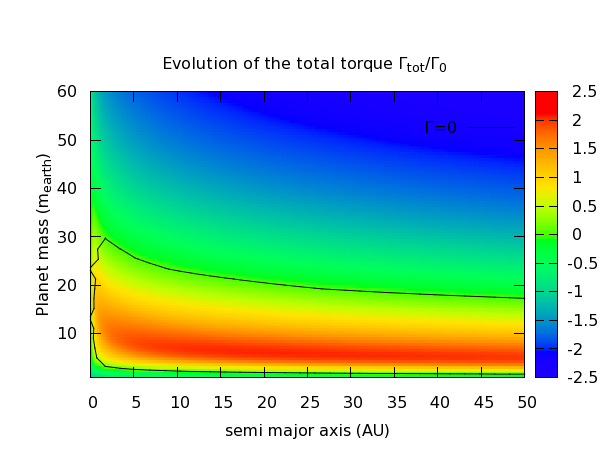
\includegraphics[width=0.65\linewidth]{figures/pm3d-map_plus_contour.png}
\caption{Affichage d'une carte 2D d'un fichier de donnée avec des contours en surimpression}\label{fig:map_plus_contour}
\end{figure}

\bigskip
\begin{verbatim}
set contour base; set cntrparam levels discret 0.
\end{verbatim}
On défini les niveaux des contours (ici, uniquement une ligne pour $z=0$).

\begin{verbatim}
unset surface
set table "contour.dat"
\end{verbatim}
On enlève la surface et on définit un fichier dans lequel on va stocker les données de sortie.

\begin{verbatim}
set dgrid3d 50, 50, 10
\end{verbatim}
La ligne \texttt{set dgrid3d} est dans le cas d'un fichier de données (contrairement à une fonction que l'on définierait directement dans gnuplot ($f(x,y) = x*x - y*y$ par exemple). Comme on veut tracer et faire un contour d'un tableau de donnée, on a besoin de convertir ce tableau de donnée en grille dans un premier temps.

\begin{attention}
L'échantillonnage en $x$, $y$ et $z$ est crucial pour avoir un rendu correct des contours. Ce maillage est à adapter. J'ai eu des problèmes pendant 2 jours parce que je ne définissais pas du tout de maillage (il en fait un par défaut je suppose) et je pestais parce que je n'avais pas de contours du tout (alors que je savais qu'il existait une ligne $z=0$).
\end{attention}


\begin{verbatim}
splot 'test_total_torque.dat'
unset table
# Draw the plot
reset
\end{verbatim}
On trace le tableau de donnée \textbf{test\_total\_torque.dat}, comme on a défini \texttt{unset surface}, le tableau de donnée ne sera pas affiché. Une grille 3D est alors effectuée (\texttt{set dgrid3d 50, 50, 10}) et un contour de cette grille pour les valeurs définies est recherché (\texttt{set cntrparam levels discret 0.}). Le résultat est alors stocké dans \textbf{contour.dat}.

On désactive alors la table, et on double les lignes blanches (apparemment nécessaires à l'affichage correct des contours pour la suite. J'ai testé et ça semble fonctionner même sans ça), ces nouvelles données sont alors stockées dans \textbf{contour1.dat}.

Un \texttt{reset} est alors effectué pour pouvoir tracer la courbe pour de bon. 

\begin{attention}
Les contours seront ceux du fichier \textbf{test\_total\_torque.dat}, celui ci doit bien évidemment être le même que celui qui sera affiché en même temps que le contour dans la 2\ieme partie du script, sinon ça n'a pas de sens. 
\end{attention}


\begin{verbatim}
set terminal wxt enhanced
set xlabel "semi major axis (AU)"
set ylabel "Planet mass (m_{earth})" center
set title "Evolution of the total torque {/Symbol G}_{tot} "
\end{verbatim}
On définit le terminal et les titres. Les labels ne sont bien entendu pas obligatoire.

\begin{verbatim}
set pm3d map
set pm3d explicit
\end{verbatim}
On définit le fait qu'on peut un plot 3D, affiché uniquement en 2D avec la variation en $z$ affichée selon une palette de couleur. On veut que les plots soient explicitement spécifiés comme 3D, ceci nous permet d'afficher les contours simplement en 3D (des lignes noires quoi). 

\begin{verbatim}
set palette rgbformulae 22,13,-31
\end{verbatim}
On change la palette de couleur (c'est un arc en ciel, plus pratique pour discerner les couleurs, et donc les valeurs associées).

\begin{verbatim}
splot 'test_total_torque.dat' with pm3d notitle,\
      'contour.dat' with line lt -1 title '{/Symbol G} = 0'
\end{verbatim}
On affiche les données de \textbf{test\_total\_torque.dat} et le contour \textbf{contour1.dat} (qui est censé correspondre à \textbf{test\_total\_torque.dat} sinon ça n'a pas de sens). La partie \texttt{title ''} permet d'éviter l'affichage du nom du fichier sur la courbe.

\begin{verbatim}
pause -1 # wait until a carriage return is hit
\end{verbatim}
Le graphique restera affiché à l'écran tant qu'on n'a pas appuyé sur la touche \touche{Entrée} (et ainsi continuer le script)

\begin{verbatim}
set terminal pngcairo enhanced
set output 'total_torque.png'
replot # pour générer le fichier d'output
\end{verbatim}
On stocke le graphique dans un fichier \textbf{.png}

\begin{verbatim}
!rm contour.dat
\end{verbatim}
On efface le fichier temporaire qui a été créé pour stocker le contour.

\section{Exporter la courbe}\label{sec:terminal}
Le principe de gnuplot est de sélectionner un terminal où envoyer les données du graphique. par défaut, ce terminal est \textbf{x11}. 

Pour définir un terminal il suffit de rentrer
\begin{verbatim}
set terminal x11
\end{verbatim}
Cette dernière commande est la commande par défaut, celle qui permet d'afficher les graphiques à l'écran.

Dans le mode interactif de gnuplot, on accède à la liste des terminaux via
\begin{verbatim}
help terminal
\end{verbatim}


\subsection{Affichage avancé à l'écran}
Voici un terminal que j'aime bien parce qu'il permet de zoomer sur la courbe notamment

\begin{verbatim}
set terminal wxt enhanced
\end{verbatim}

\begin{remarque}
\texttt{enhanced} permet une gestion avancée des textes, notamment avec indice et exposant. Pour plus de détails voir \refsec{sec:enhanced}.
\end{remarque}


\subsection{Fichier pdf}
\begin{verbatim}
set terminal pdfcairo
set output 'graphique.pdf'
replot
\end{verbatim}

\begin{remarque}
Le \texttt{replot} n'est utile que si la courbe a déjà été affichée (à l'écran par exemple).
\end{remarque}

\subsection{fichier svg}
\begin{verbatim}
set terminal svg rounded size 450,360
set output 'graphique.svg'
replot
\end{verbatim}

\subsection{fichier png}
\begin{verbatim}
set terminal pngcairo
set output 'graphique.png'
replot
\end{verbatim}


\section{Les options}
\subsection{label}
\begin{verbatim}
set xlabel "axe des abscisses"
set ylabel "axe des ordonnées"
\end{verbatim}

\subsection{échelle logarithmique}
\begin{verbatim}
set logscale x
set logscale y
\end{verbatim}

\subsection{grille}
\begin{verbatim}
set grid
\end{verbatim}
affiche une grille sur les traits majeurs.

Pour afficher aussi la grille mineure, il faut utiliser à la place 
\begin{verbatim}
set mxtics 5
set mytics 5
set grid xtics ytics mxtics mytics linetype -1, 0
\end{verbatim}
\texttt{set mxtics 5} signifie que la grille mineure horizontale va subdiviser un grand intervalle en 5 sous intervalles. Si l'intervalle est de 0 à 10, il y aura donc des traits mineurs pour 2, 4, 6 et 8. 

\texttt{linetype -1, 0} signifie que la grille majeure sera affichée avec un type de ligne \textbf{-1} (ligne noire continue) et la grille mineure avec le type de ligne \textbf{0}, c'est à dire une ligne pointillée noire.

\begin{attention}
La virgule dans \texttt{linetype -1, 0} est la seule virgule de la ligne, et sépare les styles de ligne pour grille majeure et mineure. Il n'y a pas d'autre virgule dans la ligne (sauf autre option en nécessitant éventuellement).
\end{attention}




\subsection{Forcer un zoom}
\begin{verbatim}
set xrange [0:5]
\end{verbatim}

\subsection{Style de courbe}
La commande \textbf{test}, donnée à \textbf{gnuplot}, permet d'afficher un graphique avec les différentes possibilités comme le montre \reffig{fig:styles}. Je n'ai pas réussi à récupérer le code source de la commande \textbf{test} par contre. Cette figure permet de voir les différentes possibilités, en particulier en matière de style de point ou de ligne. L'utilisation des paramètres pour contraindre le style d'affichage est détaillé dans les sous-sections suivantes.

\begin{figure}[htb]
\centering
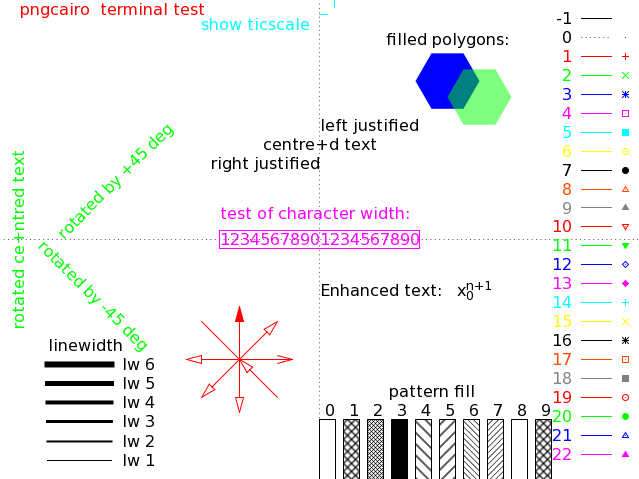
\includegraphics[width=0.65\linewidth]{figures/test_styles.png}
\caption{Résultat de la commande \textbf{test} dans le cas du terminal \textbf{pngcairo} : affichage des différents styles et personnalisations graphiques offertes par gnuplot. Pour les styles de lignes, de points, types etc, le numéro pour avoir le style correspondant est à gauche, mais ce n'est pas la même commande selon qu'on veut un style de ligne (linestyle) ou de points (pointtype)}\label{fig:styles}
\end{figure}

Notez que cette figure a des rendus différents suivant le terminal choisi. Je n'ai pas réussi à avoir le résultat pour un terminal .pdf par exemple. Ou plutôt, impossible d'ouvrir le .pdf ensuite.

\bigskip

Il y a principalement deux styles d'affichage, la ligne, et les points. La différence majeure est que les points correspondent aux points des données, alors que la ligne (même pointillée) relie entre elle les points et ne se préoccupe pas de la densité de points. S'il y a très peu de points, vous verrez clairement les traits reliant les points mais sinon, vous pourrez avoir une idée très vague de l'échantillonnage, et surtout de la variation de celui-ci le long de la courbe.

\subsubsection{Les lignes}
Pour afficher une courbe à l'aide d'une ligne : 
\begin{verbatim}
plot 'test_opacity.dat' using 1:2 with lines
\end{verbatim}\index{line}

La version compliquée est :
\begin{verbatim}
plot 'test_opacity.dat' using 1:2 with lines linetype 0 linewidth 3 
\end{verbatim}\index{linetype}\index{line}\index{linewidth}
où \textbf{linetype} permet de sélectionner la couleur de la ligne (\texttt{linetype 0} est un cas particulier pour avoir une ligne pointillée noire) et \textbf{linewidth} permet de spécifier la largeur de la ligne, dont la valeur n'est pas forcément entière (\texttt{linewidth 0.4} ou \texttt{linewidth 2.5} fonctionnent).

\subsubsection{Les points}
Pour afficher les points correspondant à une liste de données (sans les relier entre elles) :
\begin{verbatim}
plot 'test_opacity.dat' using 1:2 with points
\end{verbatim}\index{point}

Une version un peu plus complexe est :
\begin{verbatim}
plot 'test_opacity.dat' using 1:2 with points linetype -1 pointtype 2 linewidth 3
\end{verbatim}\index{linetype}\index{point}\index{linewidth}\index{pointtype}
\textbf{linetype} permet de choisir la couleur (ici noir), \textbf{pointtype} permet de choisir le type de point (ici une croix) et \textbf{linewidth} la largeur des points. 

\begin{attention}
Le type de point \texttt{pointtype -1} est un peu particulier puisque c'est un point, mais non affecté par la taille. On ne peut pas le grossir avec \textbf{linewidth}.
\end{attention}


\subsection{Texte avancé}\label{sec:enhanced}
Dans le terminal\footnote{Pour plus de détails sur la définition du terminal, voir \refsec{sec:terminal}} courant, lors de sa définition, il faut rajouter l'option \texttt{enhanced}

\begin{verbatim}
set terminal x11 enhanced
\end{verbatim}

\begin{attention}
Tous les terminaux ne supportent l'affichage de texte avancé (et donc l'option \textbf{enhanced})
\end{attention}


Ceci permet de faire du texte en indice, en exposant et d'accéder aux lettres grecques par exemple. 

On peut alors écrire dans le graphique \verb|x_1 + y^2| qui apparaîtra comme $x_1 + y^2$.

\begin{remarque}
Pas besoin de mettre en mode mathématique, il suffit de l'écrire comme ça.
\end{remarque}


\bigskip

Une différence importante a lieu pour l'affichage des lettres grecques : 
\begin{center}
\begin{tabular}{*{4}{|c|c|}}
\hline
ALPHABET  & SYMBOL  & ALPHABET  & SYMBOL  & alphabet  & symbol  & alphabet  & symbol \\\hline\hline
A  & A  & N  & N  & a  & $\alpha$  & n  & $\nu$\\\hline
B  & B  & O  & O  & b  & $\beta$  & o  & o\\\hline
C  & X  & P  & $\Pi$  & c  & $\chi$  & p  & $\pi$\\\hline
D  & $\Delta$  & Q  & $\Theta$  & d  & $\delta$  & q  & $\theta$\\\hline
E  & E  & R  & P  & e  & $\epsilon$  & r  & $\rho$\\\hline
F  & $\Phi$  & S  & $\Sigma$  & f  & $\phi$  & s  & $\sigma$\\\hline
G  & $\Gamma$  & T  & T  & g  & $\gamma$  & t  & $\tau$\\\hline
H  & H  & U  & Y  & h  & $\eta$  & u  & $\upsilon$\\\hline
I  & I  & V  & $\varsigma$  & i  & $\iota$  & v & $\varpi$\\\hline
J & $\vartheta$ & W  & $\Omega$ & j & $\varphi$ & w  & $\omega$\\\hline
K  & K  & X  & $\Xi$  & k  & $\kappa$  & x  & $\xi$\\\hline
L  & $\Lambda$  & Y  & $\Psi$  & l  & $\lambda$  & y  & $\psi$\\\hline
M  & M  & Z  & Z  & m  & $\mu$  & z  & $\zeta $\\\hline
\end{tabular}
\end{center}

Ainsi, pour faire la lettre minuscule $\alpha$ il faut faire : 
\begin{verbatim}
{/Symbol a}
\end{verbatim}

\begin{attention}
Ce n'est pas un anti-slash comme les habitudes \LaTeX{} pourraient nous le faire croire.
\end{attention}

\section{FAQ}
\subsection{pm3d map : l'image ne remplit pas le graphique}
\reffig{fig:map_wrong_range} montre une courbe où la carte ne rempli pas le graphique. J'ai mis du temps à trouver mais j'ai pu constater que c'était dû aux valeurs extrémales de mes données. 

\begin{figure}[htb]
\centering
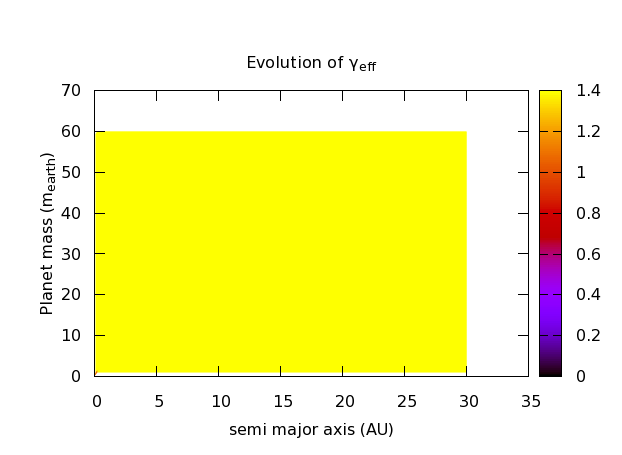
\includegraphics[width=0.65\linewidth]{figures/pm3d-map_wrong_range.png}
\caption{Exemple d'affichage incorrect de données avec \texttt{pm3d map}. Il y a des blancs sur les bords du graphique que l'on ne souhaite pas.}\label{fig:map_wrong_range}
\end{figure}

\begin{verbatim}
  0.161206   60.000000000000007      -0.65698873843863126     
\end{verbatim}
J'ai en effet \texttt{60.000000000000007} au lieu de \texttt{60}, c'est peu mais suffisant pour que gnuplot rajoute la partie 60:70 sur le graphique. 

Si vous utilisez 
\begin{verbatim}
set yrange [0:60]
\end{verbatim}
les données ayant $y=60.000000000000007$ ne seront pas affichées. La solution que j'ai utilisé est de rajouter dans mon code l'écriture du \texttt{yrange} avec les valeurs du code. 

J'obtiens alors : 
\begin{verbatim}
 set xrange [  9.99999977648258209E-003 :   50.000000000000000      ]
 set yrange [   1.0000000000000000      :   60.000000000000007      ]
\end{verbatim}

L'affichage est alors correct.

\subsection{pm3d map : mauvais affichage de la première colonne}
J'avais un affichage étrange de la première colonne de donnée, comme le montre \reffig{fig:wrong_first_column}. Ceci est dû aux données que je cherche à afficher. 

\begin{figure}[htb]
\centering
\subfloat[Bug d'affichage]{\label{fig:wrong_first_column}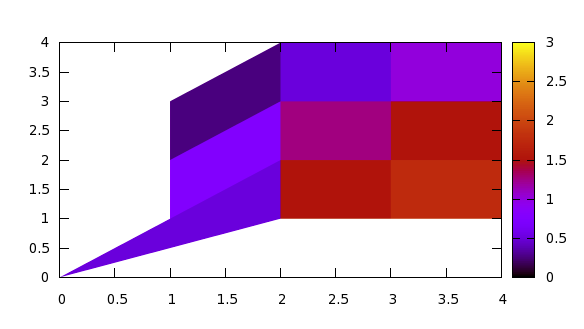
\includegraphics[width=0.48\linewidth]{figures/wrong_first_column_display.png}}\hfill
\subfloat[Affichage correct]{\label{fig:correct_first_column}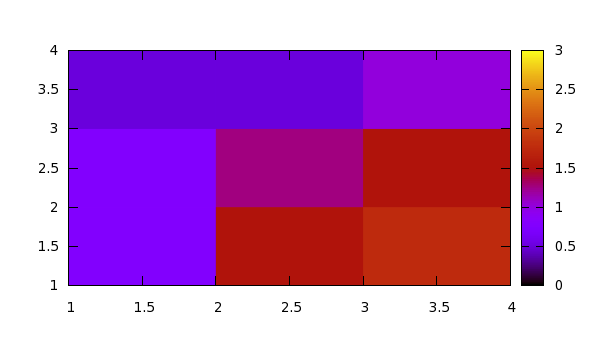
\includegraphics[width=0.48\linewidth]{figures/correct_first_column_display.png}}
\caption{Exemple d'affichage incorrect de la première colonne avec \texttt{pm3d map}}
\end{figure}

\begin{important}
Il faut que les lignes qui contiennent des commentaires ou légendes commencent par le caractère \verb|#|
\end{important}


Pour un mauvais affichage, j'ai 
\begin{verbatim}
x y z
1 1 0
1 2 1
1 3 0
1 4 2

2 1 0
2 2 2
2 3 0
2 4 0

3 1 3
3 2 1
3 3 2
3 4 0

4 1 2
4 2 1
4 3 2
4 4 0
\end{verbatim}

Pour un affichage correct il faut : 
\begin{verbatim}
#x y z
1 1 0
1 2 1
1 3 0
1 4 2

2 1 0
2 2 2
2 3 0
2 4 0

3 1 3
3 2 1
3 3 2
3 4 0

4 1 2
4 2 1
4 3 2
4 4 0
\end{verbatim}

\begin{remarque}
Les données étant affichées via : 
\begin{verbatim}
set pm3d map
splot 'test.dat'
pause -1 # wait until a carriage return is hit
\end{verbatim}

\end{remarque}



\printindex
\end{document}